%==============================================================================
% Voorbeeld gebruik documentklasse hogent-article
%==============================================================================
%
% Compileren in TeXstudio:
%
% - Zorg dat Biber de bibliografie compileert (en niet Biblatex)
%   Options > Configure > Build > Default Bibliography Tool: "txs:///biber"
% - F5 om te compileren en het resultaat te bekijken.
% - Als de bibliografie niet zichtbaar is, probeer dan F5 - F8 - F5
%   Met F8 compileer je de bibliografie apart.
%
% Als je JabRef gebruikt voor het bijhouden van de bibliografie, zorg dan
% dat je in ``biblatex''-modus opslaat: File > Switch to BibLaTeX mode.

\documentclass{hogent-article}

\usepackage{lipsum} % Voor vultekst
\usepackage{graphicx}
\graphicspath{ {./imgAnalyse/} }

%------------------------------------------------------------------------------
% Metadata over het artikel
%------------------------------------------------------------------------------

%---------- Titel & auteur ----------------------------------------------------

\PaperTitle{Invloed van moedertaal en land van geboorte op wiskundige geletterdheid}
% Dit is typisch de opdracht en het vak waarvoor dit artikel geschreven is, bv.
% ``Verslag onderzoeksproject Onderzoekstechnieken 2018-2019''
\PaperType{Verslag onderzoeksproject Onderzoekstechnieken 2020--2021}

\Authors{Isaac {Bauters}\textsuperscript{1}, Sibian {De Gussem}\textsuperscript{2}, Thomas {Dirven}\textsuperscript{3}, Bram {Krick}\textsuperscript{4}, Gaëtan {Vermaerke}\textsuperscript{5}} % Authors


% Als het hier gaat om een voorstel voor de bachelorproef, dan ben je hier
% verplicht de naam van je co-promotor in te vullen. Zoniet, dan kan je het
% leeg laten.
\CoPromotor{Thomas {Aelbrecht}}

% Contactinfo: Geef hier de contactgegevens van elke auteur van het artikel (en
% indien van toepassing ook van de co-promotor).
\affiliation{
  \textsuperscript{1} \href{mailto:isaac.bauters@student.hogent.be}{isaac.bauters@student.hogent.be}}
\affiliation{
  \textsuperscript{2} \href{mailto:sibian.degussem@student.hogent.be}{sibian.degussem@student.hogent.be}}
\affiliation{
  \textsuperscript{3} \href{mailto:thomas.dirven@student.hogent.be}{thomas.dirven@student.hogent.be}}
\affiliation{
    \textsuperscript{4} \href{mailto:bram.krick@student.hogent.be}{bram.krick@student.hogent.be}}
\affiliation{
    \textsuperscript{5} \href{mailto:gaetan.vermaerke@student.hogent.be}{gaetan.vermaerke@student.hogent.be}}


%---------- Abstract ----------------------------------------------------------

%-- \Abstract{Hier schrijf je de samenvatting van je artikel, als een doorlopende tekst van één paragraaf. Wat hier zeker in moet vermeld worden: \textbf{Context} (Waarom is dit werk belangrijk?); \textbf{Nood} (Waarom moet dit onderzocht worden?); \textbf{Taak} (Wat ga je (ongeveer) doen?); \textbf{Object} (Wat staat in dit document geschreven?); \textbf{Resultaat} (Wat verwacht je van je onderzoek?); \textbf{Conclusie} (Wat verwacht je van van de conclusies?); \textbf{Perspectief} (Wat zegt de toekomst voor dit werk?).

\Abstract{In dit onderzoek is er gepoogd antwoord te krijgen op de vraag of het hebben van een andere moedertaal, frequent een andere taal spreken of land van geboorte een invloed heeft op de wiskundige geletterdheid bij studenten in het Vlaamse hoger onderwijs. Onderzoek naar deze specifieke doelgroepen en hun schoolresultaten is nodig om onderbenutting van talent in het hoger onderwijs tegen te gaan zoals beschreven in de literatuurstudie. Voor dit onderzoek werd gebruikt gemaakt van een dataset van HoGent over wiskundige geletterdheid.


Bij de start van dit onderzoek werd een hypothese geformuleerd a.d.h.v. de beschikbare variabelen in de dataset. Later werd een literatuuronderzoek over het onderwerp geschreven na een reading group. Tenslotte werd de dataset onderworpen aan een statistische analyse in Rstudio, aan de hand van deze analyse is er een conclusie neergeschreven. Je kan het volledige verloop van ons onderzoek hieronder weervinden.
}

% --Bij de sleutelwoorden geef je het onderzoeksdomein, samen met andere sleutelwoorden die je werk beschrijven.

%---------- Onderzoeksdomein en sleutelwoorden --------------------------------

\Keywords{ Wiskundige geletterdheid; Moedertaal; Geboorteland; Thuistaal}
\newcommand{\keywordname}{Sleutelwoorden} % Defines the keywords heading name

%---------- Titel, inhoud -----------------------------------------------------

\begin{document}

\flushbottom % Makes all text pages the same height
\maketitle % Print the title and abstract box
\tableofcontents % Print the contents section
\thispagestyle{empty} % Removes page numbering from the first page

%------------------------------------------------------------------------------
% Hoofdtekst
%------------------------------------------------------------------------------

\section{Inleiding}\label{sec:inleiding}

In deze literatuurstudie wordt er een antwoord gezocht op de vraag of het hebben van een andere moedertaal, frequent een andere taal spreken of land van geboorte een invloed heeft op de wiskundige geletterdheid bij studenten in het Vlaamse hoger onderwijs. Artikels werden gevonden via Google Scholar en Web of Science.

\section{Overzicht literatuur}\label{sec:overzicht-literatuur}

% Refereren naar de literatuur kan met:
% \autocite{BIBTEXKEY} -> (Auteur, jaartal)
% \textcite{BIBTEXKEY} -> Auteur (jaartal)

\subsection*{Onderbenutting van talent}

Onderbenutting van talent heeft sinds de jaren zestig van de vorige eeuw een belangrijke rol gespeeld in discussies over de kwaliteit van het onderwijs. Een ijkpunt daarbij was het zogeheten Talentenproject dat het Leids Sociologisch Instituut onder leiding van \textcite{VanHeek1968} uitvoerde. Hoewel onder andere omstandigheden was ook toen al de vraag in hoeverre cognitieve talenten van kinderen ten volle tot ontplooiing in het onderwijs konden komen. De sociale achtergrond (het sociale netwerk en culturele hulpbronnen van het gezin) bleken naast aanleg een beduidende rol te spelen in de schoolcarri\`eres van leerlingen~\autocite{FrederikRiemersma2007}.

Bij onderzoek in Vlaanderen hebben Opdenakker en Hermans, volgens \textcite{Agirdag2014}, op basis van de LOSO1 gegevens berekend dat op het einde van het lager onderwijs \'e\'en op vier allochtone (Maghrebijnse en Turkse) leerlingen een vertraging van een minstens een jaar heeft oplopen, terwijl slechts \'e\'en op tien autochtone leerlingen zijn blijven zitten (verschil = 15\%). Ook op vlak van studiekeuze is er een verschil, waar slechts 21\% van de autochtonen leerlingen in het beroepsonderwijs (BSO) afstuderen, is dat 50\% voor allochtone leerlingen (verschil = 29\%). Op basis van de PISA 2009 gegevens werd berekend dat autochtone leerlingen in het Vlaamse secundair onderwijs beter presteren dan nieuwkomers op vlak van leesvaardigheid (verschil = 64 PISA punten), op vlak van wiskunde (verschil = 62), en op vlak van wetenschappen (verschil = 66). Ook tweede generatie leerlingen scoren significant slechter dan autochtone leerlingen: verschillen voor leesvaardigheid, wiskunde en wetenschappen zijn respectievelijk 76, 84 en 95 PISA punten~\autocite{Agirdag2014}.

\subsection*{De schoolse prestaties van migrantenleerlingen in Vlaanderen}

De kinderen van migrantenfamilies die verhuisd zijn naar Belgi\"e hebben het niet makkelijk om zich snel aan te passen aan het Belgische onderwijssysteem en het niveau ervan.

Dit blijkt uit het thematische OESO-rapport over de schoolse prestaties van migrantenleerlingen, dat verscheen in 2006, dat in Vlaanderen flink wat stof deed opwaaien. Uit het rapport bleek dat leerlingen met een buitenlandse herkomst in heel wat landen significant onder de autochtone leerlingengroep presteren. Vlaanderen bleek op dit punt de slechtste leerling van de klas: in geen enkel ander land is het puntenverschil op de schaal voor wiskundige geletterdheid tussen autochtone en allochtone leerlingen zo groot als in Vlaanderen.

Bovendien blijkt de mate waarin leerlingen van buitenlandse herkomst benadeeld zijn op het vlak van hun sociaaleconomische situatie ook een invloed te hebben op hun gemiddelde prestaties. In landen waar de sociaaleconomische status van migrantenfamilies eerder laag is, zal de prestatiekloof tussen leerlingen met en zonder migratieachtergrond groter zijn. Vlaanderen is \'e\'en van die voorbeelden waar de migrantengroep gemiddeld een lagere sociale status bezit dan de autochtone bevolking.

Van de overige factoren die een invloed uitoefenen op de prestatieverschillen tussen autochtone leerlingen en leerlingen van buitenlandse herkomst, blijkt de thuistaal van leerlingen in het Vlaamse onderwijssysteem een zeer sterke medi\"erende factor. Zowel bij autochtone leerlingen als bij leerlingen met een buitenlandse herkomst heeft de thuistaal een grote impact op hun gemiddelde prestatie. Enerzijds halveert het prestatieverschil tussen autochtone leerlingen en leerlingen van buitenlandse herkomst, wanneer deze laatste groep thuis Nederlands of een Vlaams dialect spreekt.

Daarenboven presteren de Vlaamse leerlingen van buitenlandse herkomst die thuis Nederlands of een dialect spreken, op hetzelfde niveau als de autochtone leerlingen die thuis een andere taal spreken. Net zoals de Vlaamse anderstalige autochtone leerlingen presteren de leerlingen van buitenlandse herkomst die thuis Nederlands of een Vlaams dialect spreken gemiddeld op het derde vaardigheidsniveau van wiskundige geletterdheid, terwijl de anderstalige leerlingen van buitenlandse herkomst gemiddeld op het tweede niveau blijven hangen (met een gemiddelde prestatie van 435 punten)

Ten slotte blijken ook de school- en studie-``keuze'' van de migrantenleerlingen hun gemiddelde prestaties te be\"{\i}nvloeden~ %\autocite{Demeyer2008}.

\subsection*{Eentalig taalbadonderwijs vs. meertalig onderwijs}

\enquote{Wanneer het over gelijke onderwijskansen gaat, wordt een taalbad beschouwd als de ultieme methode. Het taalbadmodel is nagenoeg de enige manier waarmee scholen vandaag de dag omgaan met anderstalige leerlingen}, aldus \textcite{MaartenHermans2010}. Het taalbadmodel is primair gericht op het aanleren van de dominante taal, in casu, het Nederlands. Men gaat er immers van uit dat een betere beheersing van de Nederlandse taal, betere onderwijsprestaties met zich meebrengt. Deze taalbadmethode is niet vrij van kritiek gebleven. Namelijk, hoe meer schooltijd anderstalige leerlingen spenderen aan het leren van het Nederlands op zich, hoe minder tijd ze over hebben om leerinhouden zelf te leren. Wanneer leerlingen uit reguliere klassen genomen worden, gaan de reguliere lessen immers gewoon door. Taallessen zouden ook buiten de schooluren kunnen georganiseerd worden, maar zou dan weer minder tijd voor huiswerk kunnen betekenen.

Meertalig onderwijs (of het immersie-model) is een alternatieve aanpak om anderstalige leerlingen te onderwijzen. De verschillende vormen van meertalig onderwijs hebben als gemeenschappelijke kenmerk dat de moedertaal van anderstalige leerlingen niet wordt uitgesloten, maar gevaloriseerd wordt als een onderdeel van het curriculum.

\textcite{Agirdag2014} definieerde drie redenen waarom het valoriseren van de moedertaal tot betere onderwijsprestaties zou leiden:
%toevoegen van nummers 1-3)
\begin{itemize}
    \item Volgens de afhankelijkheidshypothese van Jim Cummins (1979) is taalvaardigheid in de moedertaal (T1) gerelateerd aan taalvaardigheid in een later aangeleerde taal (T2). Leertijd investeren in de moedertaal van anderstalige leerlingen zou daarom het aanleren van het Nederlands niet verhinderen, maar net stimuleren.

    \item Het uitsluiten van de moedertaal van de school kan een negatieve invloed hebben op het welbevinden van de leerlingen, en onderzoek wijst uit dat leerlingen zich meer thuis voelen op school waar ze hun moedertaal kunnen spreken. Een verbeterd schoolwelbevinden kan dan resulteren in betere onderwijsprestaties.

    \item Uit onderzoek met hersenscans blijkt dat tweetalige leerlingen meer hersenactiviteit vertonen, wat zou betekenen dat het stimuleren van tweetaligheid ook het leervermogen van de leerlingen zou bevorderen.
\end{itemize}

\subsection*{Invloed van thuistaal van de jongeren op wiskundige geletterdheid}

\enquote{Uit de analyse van de PISA resultaten (OECD, 2013; OECD, 2016) bleek dat jongeren die een andere thuistaal hebben dan het Nederlands doorgaans slechter scoorden op vlak van financiële geletterdheid omdat kennis van het Nederlands zeer sterk gecorreleerd is met andere vaardigheden, zoals wiskundige geletterdheid en leesvaardigheid. Het is mogelijk dat jongeren die thuis een andere taal spreken dan het Nederlands een andere vorm van financiële educatie meekrijgen van hun ouders}, aldus \textcite{Cooreman2018}. Over de exacte invloed van thuistaal op wiskundige geletterdheid werden geen bronnen gevonden, wat doet vermoeden dat hier nog niet veel onderzoek naar gedaan is.

\subsection*{Besluit literatuurstudie}

Kan er besloten worden dat het hebben van een andere moedertaal, frequent een andere taal spreken of land van geboorte, een invloed heeft op de wiskundige geletterdheid bij studenten in het Vlaamse hoger onderwijs? Deze vraag staat centraal in dit werk. Het antwoord hierop is eenduidig en simpel: ja, deze factoren hebben een invloed op de wiskundige geletterdheid. Zowel nieuwkomers als tweede generatie leerlingen scoren significant slechter dan autochtone leerlingen, blijkt uit onderzoek van PISA: verschillen voor leesvaardigheid, wiskunde en wetenschappen zijn respectievelijk 76, 84 en 95 PISA punten volgens \textcite{Agirdag2014}. Wij hopen met dit onderzoek duidelijk te kunnen maken dat het hebben van een moedertaal een duidelijke en grote impact heeft op de wiskundige geletterdheid en ook op de schoolresultaten.

\section{Methodologie}\label{sec:methodologie}

De proefpersonen zijn de 217 studenten Toegepaste informatica aan HoGent academiejaar 2019--2020. In deze enqu\^ete werd vooral gepeild naar de kwalitatieve en kwantitatieve factoren die volgens de studenten zelf een invloed kunnen hebben op wiskundige geletterdheid. Ook werd hen gevraagd de resultaten op enkele vakken in de opleiding mee te delen. De dataset bevat 217 observaties van 122 variabelen, 19 van hen waren niet-Nederlandstaligen. Voor het literatuuronderzoek werden er wetenschappelijke artikelen gezocht in Google Scholar en Web Of Science.

\section{Experimenten}\label{sec:experimenten}

Vorig academiejaar hebben de studenten toegepaste informatica aan HoGent meegewerkt aan het verzamelen van de nodige data om dit onderwerp verder te kunnen onderzoeken. De studenten namen deel aan een toets die naar de wiskundige geletterdheid peilt. Ook werd door hen een enqu\^ete samengesteld die alle studenten hebben ingevuld. Daarnaast is hen ook gevraagd de resultaten op enkele vakken in de opleiding mee te delen. De begeleiders hebben alle deze resultaten geanonimiseerd en samengevoegd tot \'e\'en grote dataset. Aan de hand van deze dataset werd er door onze onderzoeksgroep een hypothese opgesteld.

\section{Analyse resultaten}\label{sec:analyse-resultaten}

Het eerste wat opvalt bij het bekijken van de boxplot van Figuur \ref{fig:1} is de verhouding tussen Nederlandstaligen en anderstaligen. De anderstaligen zijn slechts in kleine aantallen vertegenwoordigd. Men moet dus extra kritisch zijn bij het nemen van conclusies uit deze data.

De resultaten van de wiskundetoets waren sterk gelijkend voor de vragen over 1\textsuperscript{ste} graads wiskunde (Test Q01-Q05) en 2\textsuperscript{de} graads wiskunde (Test Q06-Q10), deze worden verder niet besproken. Pas bij de resultaten van de 3\textsuperscript{de} graads wiskunde oefeningen, Test Q11-Q15, zijn er verschillen merkbaar in de grafiek, zie Figuur \ref{fig:2}. Bij de boxplots voor 1\textsuperscript{ste}, 2\textsuperscript{de} en 3\textsuperscript{de} graads wiskunde is steeds veel overlap te zien, dit wijst er meestal op dat er geen verband is.

\begin{figure}
 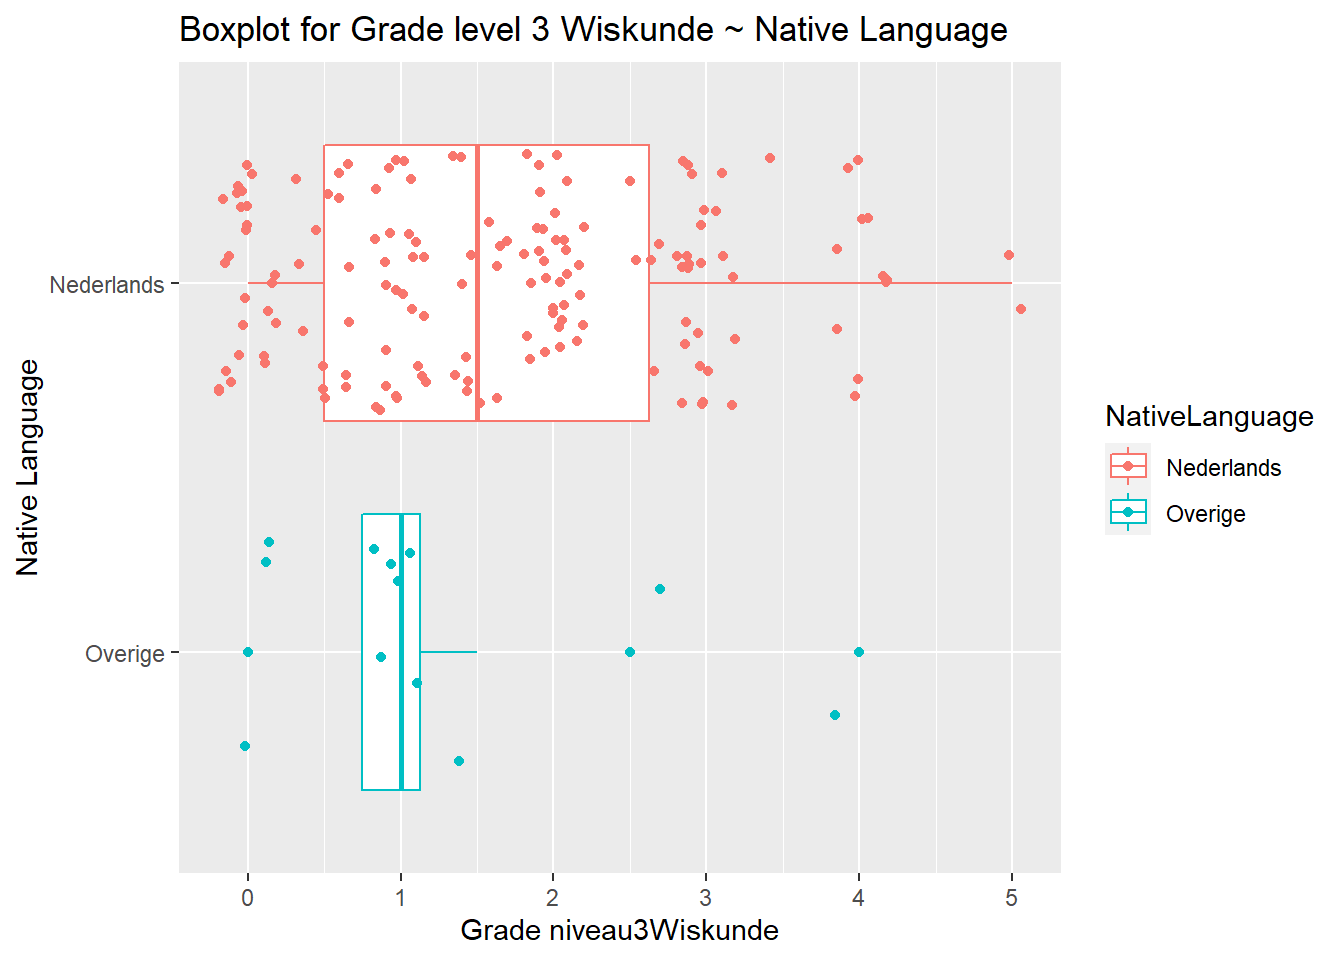
\includegraphics[width=\linewidth]{Boxplot-Niveau3Wiskunde-NativeLanguage.png}
 \caption{\label{fig:1} 3\textsuperscript{de} graads wiskunde i.f.v. Moedertaal (Boxplot)}
\end{figure}


\begin{figure}
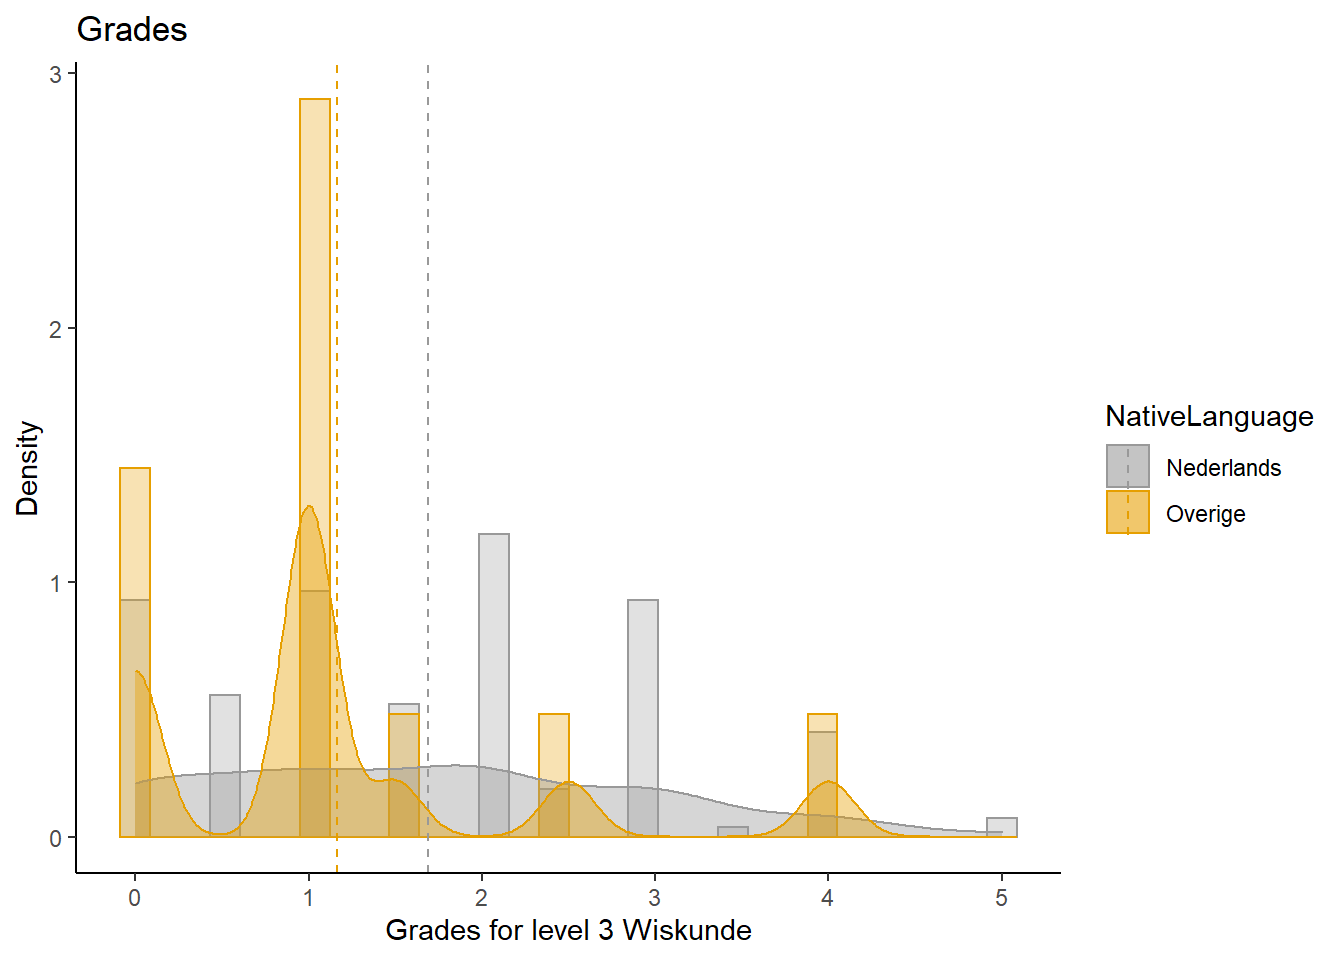
\includegraphics[width=\linewidth]{Histogram-Niveau3Wiskunde-NativeLanguage.png}
\caption{\label{fig:2} 3\textsuperscript{de} graads wiskunde i.f.v. Moedertaal}
\end{figure}

De boxplot van Figuur \ref{fig:3} illustreert de resultaten van Math4IT i.f.v.\ de Moedertaal, deze toont weer veel overlapping. De grafiek in Figuur \ref{fig:4} die hoort bij de boxplot uit Figuur \ref{fig:3} toont aan dat de wiskundige geletterdheid niet lijkt af te hangen van de moedertaal. Bij studenten met Nederlands als moedertaal zijn er meer uitschieters waar te nemen, zowel links als rechts. Dit is te verklaren omdat zij in grotere aantallen aanwezig zijn in onze steekproef. Het Q2 bij studenten met overige talen als moedertaal begint bij een iets lagere score dan het Q2 bij de Nederlandstalige studenten. Het Q3 van beiden overlappen elkaar, net als hun mediaan.

\begin{figure}
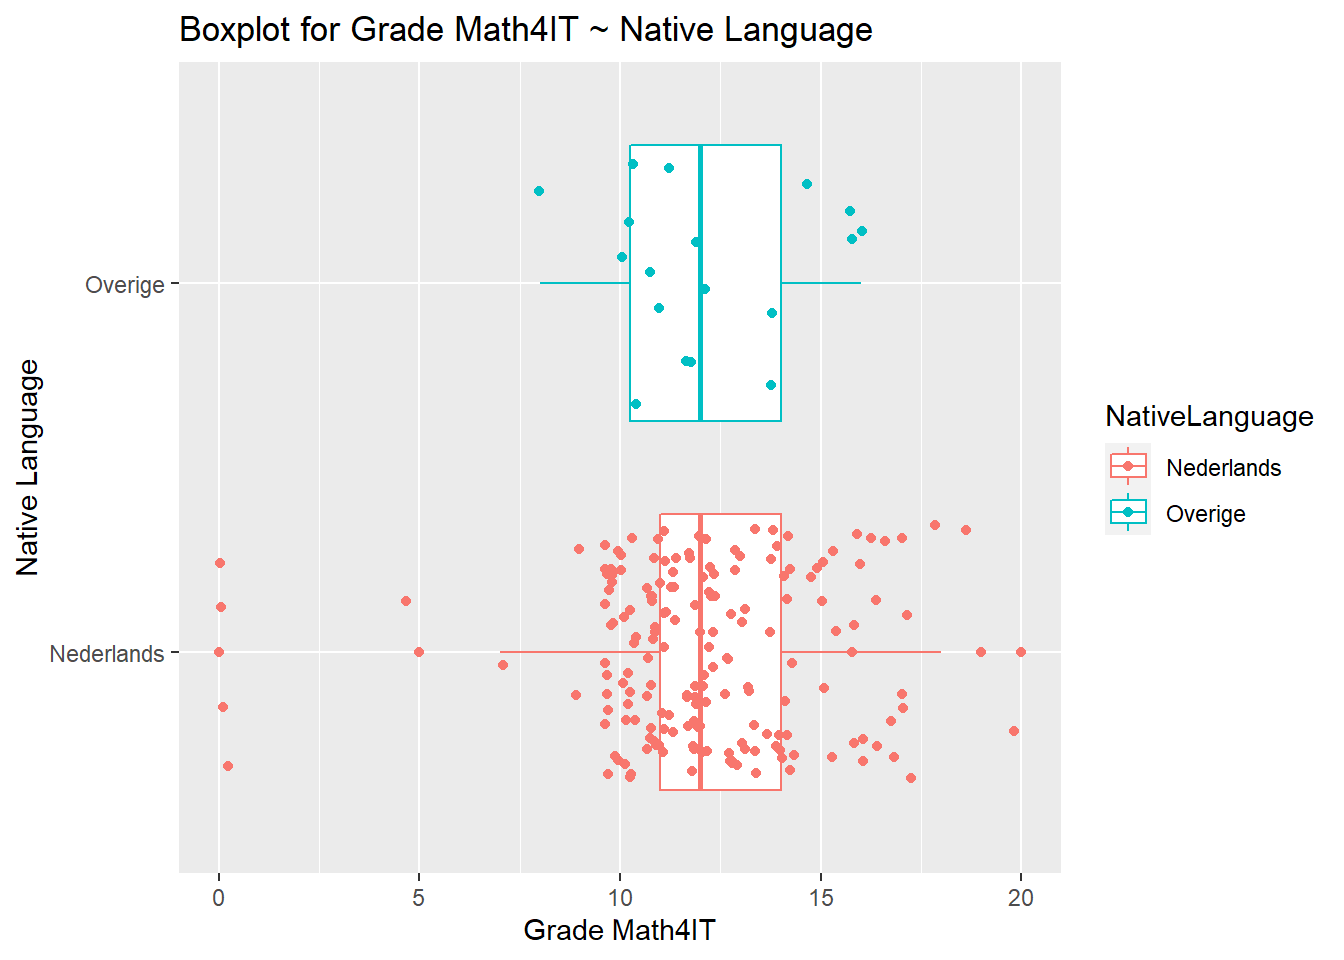
\includegraphics[width=\linewidth]{Boxplot-GradeMath4IT-NativeLanguage.png}
\caption{\label{fig:3} Score Math4IT i.f.v. Moedertaal (Boxplot)}
\end{figure}

\begin{figure}
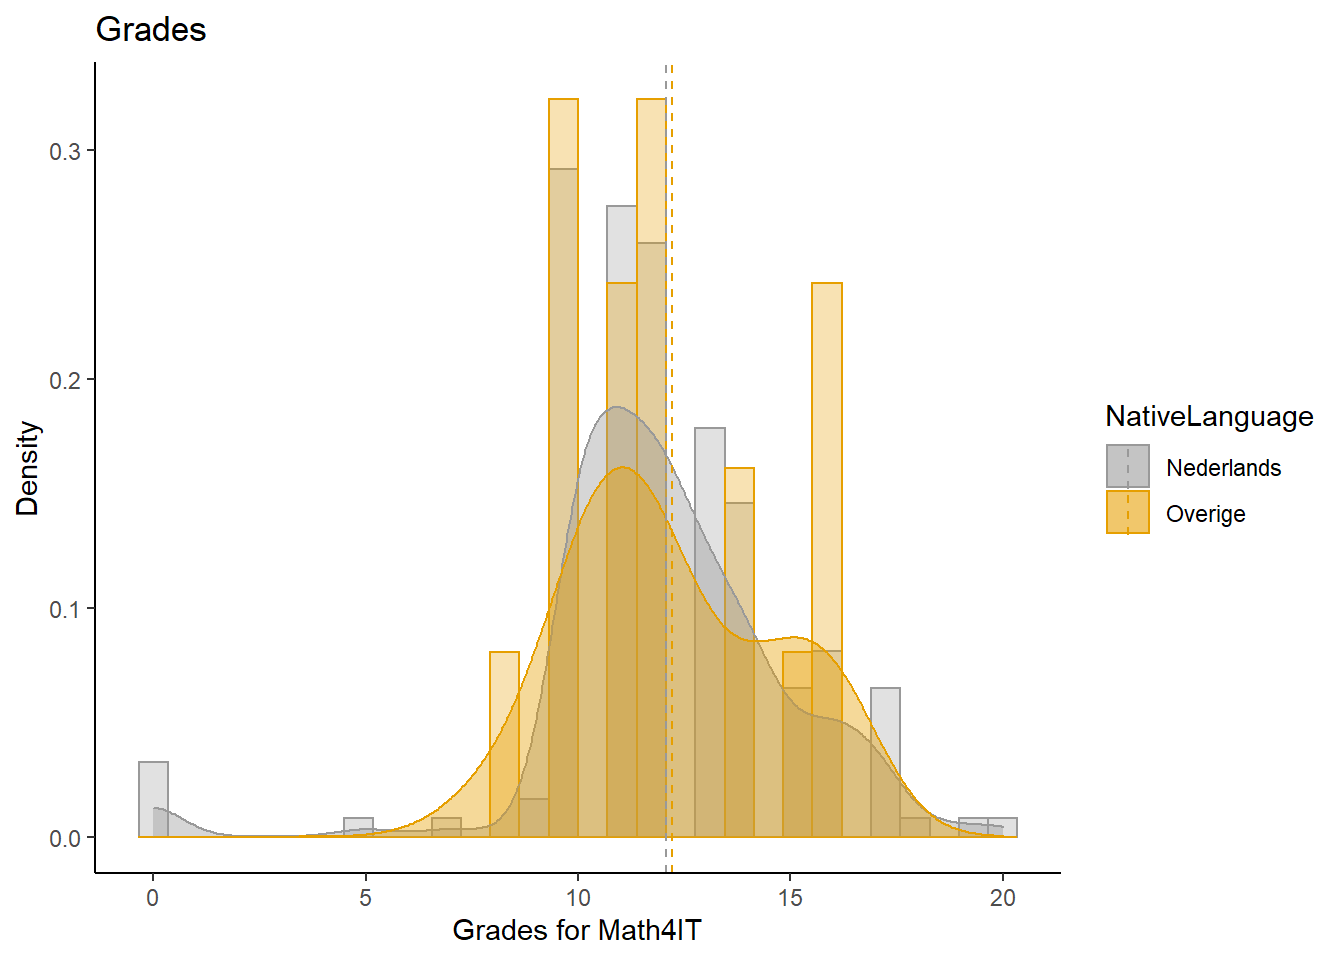
\includegraphics[width=\linewidth]{Histogram-GradeMath4IT-NativeLanguage.png}
\caption{\label{fig:4} Score Math4IT i.f.v. Moedertaal}
\end{figure}

De vlakdiagrammen op Figuur \ref{fig:5} zijn zeer gelijklopend voor de data met geboorteland als afhankelijke variabele. Dit wijst in de richting dat er geen verband zou mogen zijn tussen de wiskundige geletterdheid en het geboorteland.

\begin{figure}
    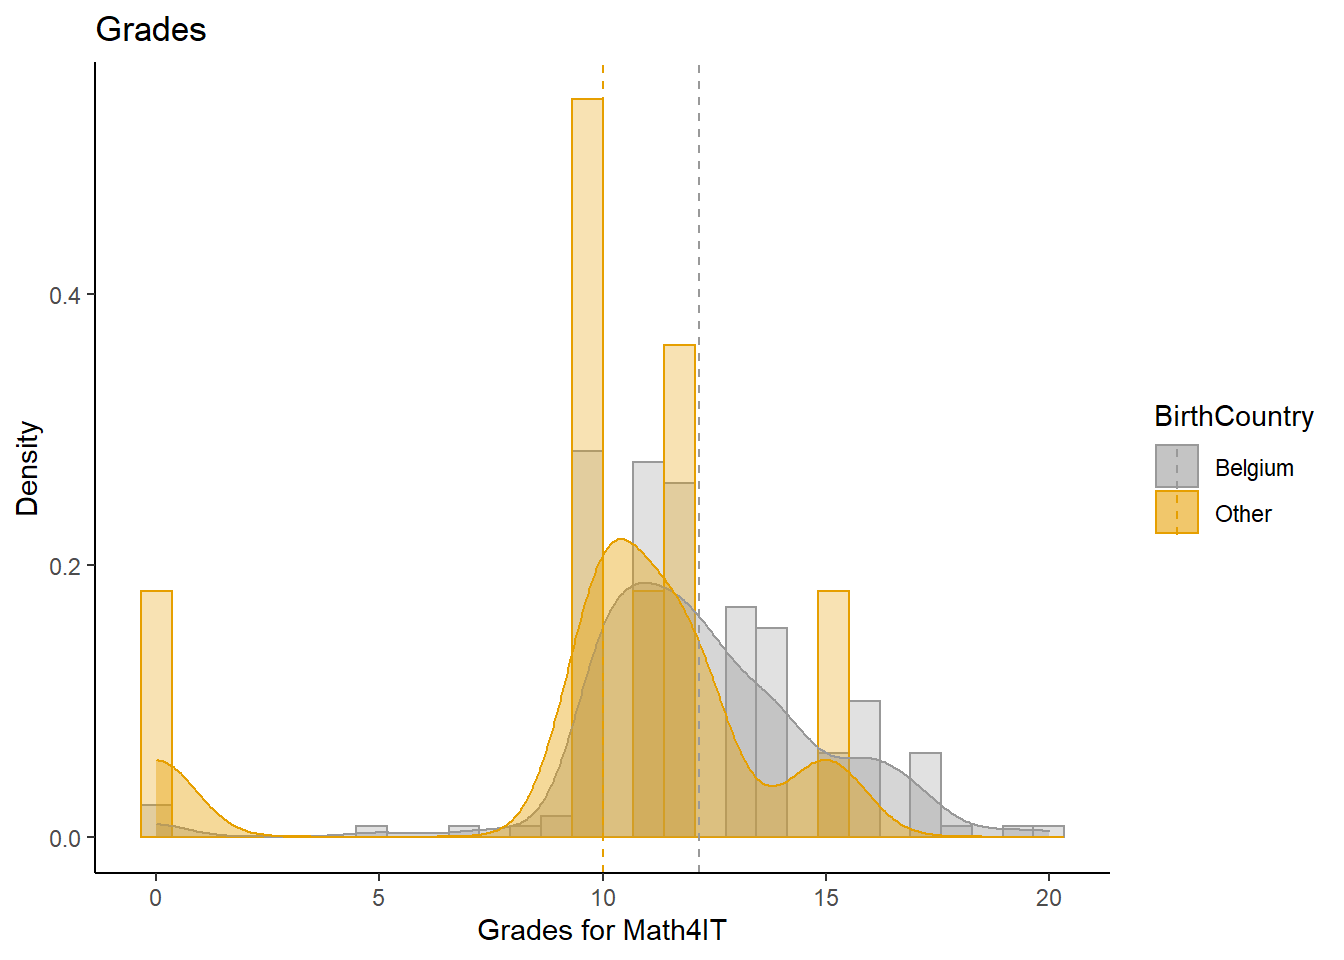
\includegraphics[width=\linewidth]{Histogram-GradeMath4IT-BirthCountry.png}
    \caption{\label{fig:5} Score Math4IT i.f.v. Geboorteland}
\end{figure}

Op de grafiek van Figuur \ref{fig:6}, waar het thuis spreken van Nederlands de onafhankelijke variabele is lijkt het moeilijker om conclusies te trekken. Het aantal studenten dat thuis geen Nederlands spreekt scoort erg hoog, ook zijn er enkelingen die heel wat lager scoren. Dit valt te verklaren omdat dit slechts een kleine groep uit de steekproef is waardoor zij een grote invloed op de visualisatie van de data kunnen hebben.

\begin{figure}
    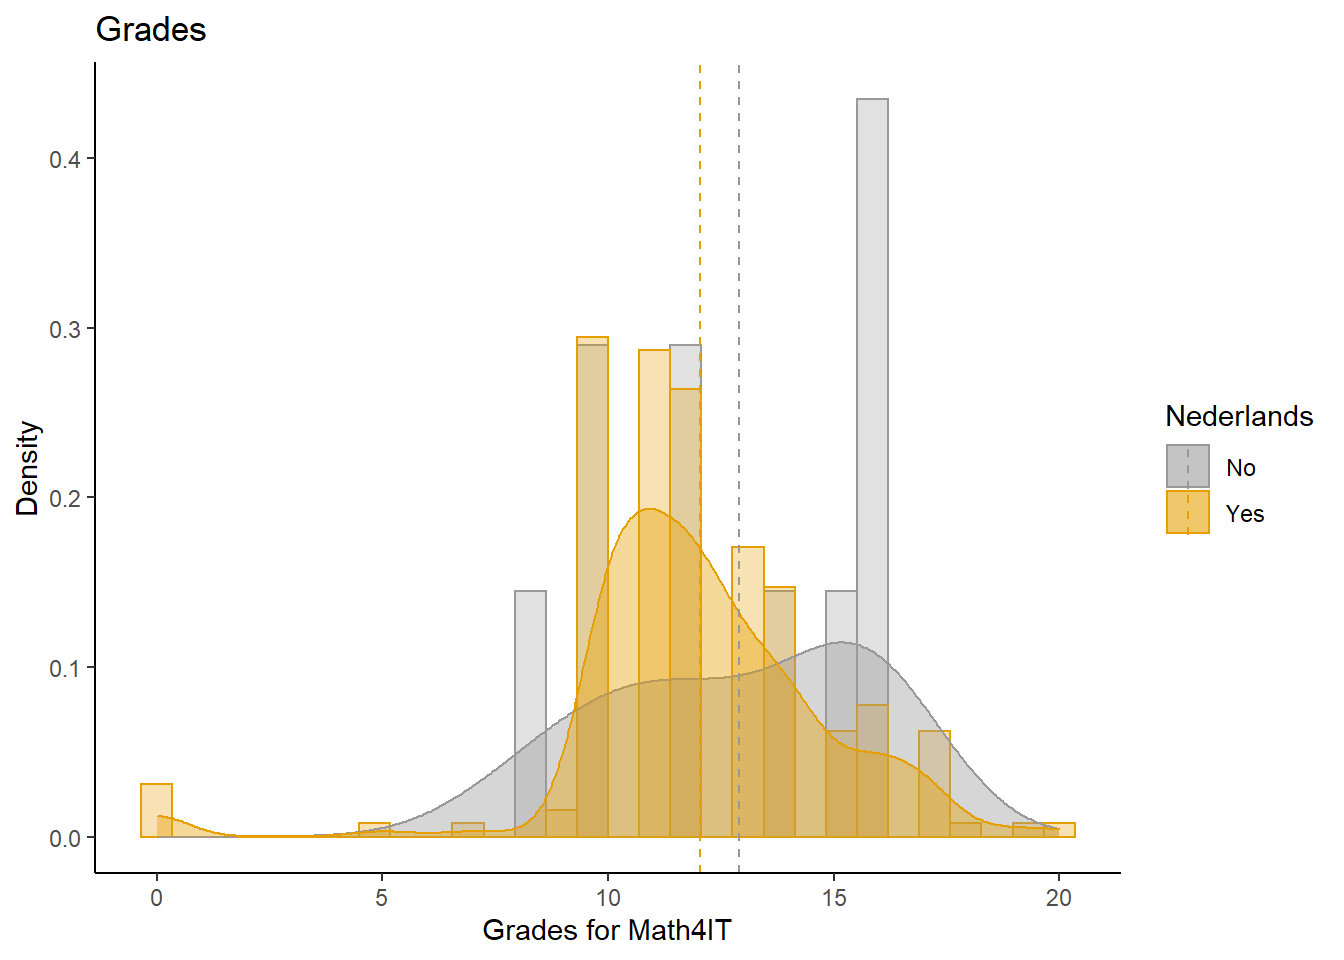
\includegraphics[width=\linewidth]{Histogram-GradeMath4IT-DutchAtHome.png}
    \caption{\label{fig:6} Score Math4IT i.f.v. Thuis Nederlands Spreken}
\end{figure}

Als laatste stap van de analyse hebben we t-testen uitgevoerd, waarbij alle gekozen kwalitatieve en kwantitatieve variabelen getest zijn t.o.v.\ elkaar. Aangezien voor alle combinaties geldt dat de p-waarde groter is dan het significantieniveau, dat 5\% of 0,05 bedraagt, kunnen we concluderen dat voor geen enkele combinatie de oorspronkelijk hypothese H0 mag verworpen worden. Dit toont aan dat er geen duidelijk verband is tussen de variabelen.

\section{Conclusie}\label{sec:conclusie}

Bij aanvang van dit onderzoek gingen we ervan uit dat een taalbarri\`ere een negatieve impact zou hebben op de wiskundige geletterdheid van Vlaamse studenten. Uit onze data bleek echter dat een dergelijke negatieve impact niet aan te tonen is met onze steekproef.

De steekproef die werd gebruikt voor ons onderzoek is geen perfecte representatie, de steekproefgrootte bedraagt ongeveer 220 personen, waarvan er maar een twintigtal geen Nederlands hebben als moedertaal.

Bij de boxplots is steeds veel overlap te zien, dit wijst er meestal op dat er geen verband is. Ook de t-testen wijzen deze richting uit, waarbij voor geen enkele combinatie de oorspronkelijke hypothese H0 verworpen mag worden. Al deze factoren samen bewijzen onze hoofdhypothese en onderzoeksvraag:

Het hebben van een andere moedertaal, frequent een andere taal spreken of land van geboorte, heeft weinig tot geen invloed op de wiskundige geletterdheid bij studenten in het Vlaamse hoger onderwijs.

Een vervolgonderzoek is nodig dat nagaat of het percentage studenten met een andere moedertaal dan Nederlands representatief is voor Vlaanderen. Hiermee wordt bedoeld dat het percentage jongeren met een andere moedertaal dan Nederlands in Vlaanderen ongeveer gelijk moet zijn met het percentage studenten met een andere moedertaal dan Nederlands. Indien uit dit onderzoek zou blijken dat deze percentages onderling sterk verschillen zou men kunnen besluiten dat het hebben van een andere moedertaal toch een impact heeft op de studiekansen van deze jongeren en daarmee dus ook een impact op hun wiskundige geletterdheid.

%------------------------------------------------------------------------------
% Referentielijst
%------------------------------------------------------------------------------
% TODO: de gerefereerde werken moeten in BibTeX-bestand ``bibliografie.bib''
% voorkomen. Gebruik JabRef om je bibliografie bij te houden en vergeet niet
% om compatibiliteit met Biber/BibLaTeX aan te zetten (File > Switch to
% BibLaTeX mode)

\phantomsection
\printbibliography[heading=bibintoc]

\end{document}
